% Methodology write-up: formal refinement of the Metronome v4 RTL in Lean 4.
% Build: tectonic lean_methodology.tex (XeTeX), or pdflatex twice.
\documentclass[11pt,a4paper]{article}

\usepackage{iftex}
\ifXeTeX
  \usepackage{fontspec}
  \setmonofont{DejaVuSansMono.ttf}[Scale=0.85]
\else
  \usepackage[T1]{fontenc}
  \usepackage[utf8]{inputenc}
  \usepackage{lmodern}
  \DeclareUnicodeCharacter{2192}{\ensuremath{\rightarrow}}\DeclareUnicodeCharacter{2190}{\ensuremath{\leftarrow}}
  \DeclareUnicodeCharacter{2200}{\ensuremath{\forall}}\DeclareUnicodeCharacter{2203}{\ensuremath{\exists}}
  \DeclareUnicodeCharacter{2227}{\ensuremath{\wedge}}\DeclareUnicodeCharacter{2228}{\ensuremath{\vee}}
  \DeclareUnicodeCharacter{2260}{\ensuremath{\neq}}\DeclareUnicodeCharacter{2264}{\ensuremath{\leq}}
  \DeclareUnicodeCharacter{27E8}{\ensuremath{\langle}}\DeclareUnicodeCharacter{27E9}{\ensuremath{\rangle}}
  \DeclareUnicodeCharacter{2191}{\ensuremath{\uparrow}}\DeclareUnicodeCharacter{2115}{\ensuremath{\mathbb{N}}}
\fi
\usepackage[margin=25mm]{geometry}
\usepackage{amsmath,amssymb}
\usepackage{booktabs}
\usepackage{tabularx}
\usepackage{enumitem}
\usepackage{xcolor}
\usepackage{listings}
\usepackage{tikz}
\usetikzlibrary{arrows.meta,positioning,fit}
\usepackage{xurl}
\usepackage[hidelinks]{hyperref}
\urlstyle{tt}

\setlist{itemsep=2pt,topsep=4pt}

\lstdefinelanguage{Lean}{
  morekeywords={theorem,lemma,def,structure,where,by,fun,let,in,if,then,else,
    match,with,import,namespace,end,abbrev,Prop,Type,intro,exact,rw,simp,cases,
    induction,obtain,decide,bv_decide,rfl,example},
  sensitive=true,
  morecomment=[l]{--},
  morecomment=[s]{/-}{-/},
  morestring=[b]"
}
\lstset{
  language=Lean,
  basicstyle=\ttfamily\small,
  keywordstyle=\color{blue!60!black}\bfseries,
  commentstyle=\color{green!40!black}\itshape,
  stringstyle=\color{red!50!black},
  columns=fullflexible,
  keepspaces=true,
  frame=single,
  framerule=0.3pt,
  rulecolor=\color{black!30},
  xleftmargin=4pt,
  xrightmargin=4pt,
  breaklines=true,
  aboveskip=6pt,
  belowskip=6pt,
  escapeinside={(*}{*)}
}

\newcommand{\brkus}{\textunderscore\allowbreak}
\ifXeTeX\else\lstset{
  literate=
    {→}{{$\rightarrow$}}1 {←}{{$\leftarrow$}}1 {∀}{{$\forall$}}1
    {∃}{{$\exists$}}1 {∧}{{$\wedge$}}1 {∨}{{$\vee$}}1 {¬}{{$\neg$}}1
    {≠}{{$\neq$}}1 {≤}{{$\leq$}}1 {⟨}{{$\langle$}}1 {⟩}{{$\rangle$}}1
    {×}{{$\times$}}1 {↑}{{$\uparrow$}}1 {ℕ}{{$\mathbb{N}$}}1}\fi
\newcommand{\code}[1]{{\let\_\brkus\texttt{#1}}}
\emergencystretch=3em
\newcommand{\lean}[1]{\texttt{\detokenize{#1}}}

\title{Formalising a Tiny Tapeout ASIC in Lean~4:\\
  Methodology for a Whole-Chip RTL Refinement Proof of Metronome~v4}
\author{Metronome project}
\date{22 November 2026}

\begin{document}
\maketitle

\begin{abstract}
We describe how the register-transfer-level (RTL) design of Metronome~v4, a
reprogrammable protocol-emulator ASIC for the IHP 130\,nm Tiny Tapeout shuttle,
was related to an independently written executable specification in Lean~4.
The headline result, \lean{trace_refines'}, states that from reset, for every
sampled pin sequence that satisfies two stated per-cycle usage rules, the
composed chip model and the specification machine stay related on every cycle.
The relation determines all 24 output, output-enable and interrupt pins. The
proof composes per-module \emph{cuts}, each extracted mechanically from the
Yosys elaboration of the Verilog and proved equal to a hand-written
specification. It rests on Lean's three standard axioms and 96 \code{bv\_decide}
SAT certificates, and contains no \code{sorry}. We focus on the methodology:
how the RTL enters the logic, how the per-module results are composed, how
premises are discharged or kept honest, and which checks outside Lean guard the
parts the proof cannot reach. We also list the trusted base and the limitations.
\end{abstract}

\tableofcontents

%======================================================================
\section{Context and goal}

Metronome~v4 is a small multi-threaded protocol engine: four pin \emph{lines},
six hardware \emph{threads}, two cores, two streams with a capture/replay
buffer, a 480-byte latch-based configuration bank, a data RAM and program
memories (IHP SRAM macros), and an SPI host port. It is reprogrammed through
the host port. The Verilog sources are in \code{src/}, with \code{project.v}
as the chip top. The behavioural contract is \code{wiki/SPEC\_V2.md}.

Two executable references already existed. One was a Python cycle model
(\path{sim/reference/metronome2}). The other was an RTL-versus-model lockstep
bench in cocotb. Both are simulation evidence: they show agreement on the
scenarios that were run. The Lean work aimed for a statement over
\emph{all} input sequences, with every assumption written down as a Lean
hypothesis rather than left implicit.

\paragraph{Scope of the claim.} The theorem is about sampled, two-state digital
behaviour at the rising clock edge, starting from the modelled reset state. It
says nothing about analog behaviour, metastability, silicon timing or
gate-level netlists after synthesis.

%======================================================================
\section{Architecture of the proof}

The proof has five layers. Each layer has its own files, and each layer
boundary is a Lean theorem or a checked Python property.

\begin{figure}[!ht]
\centering
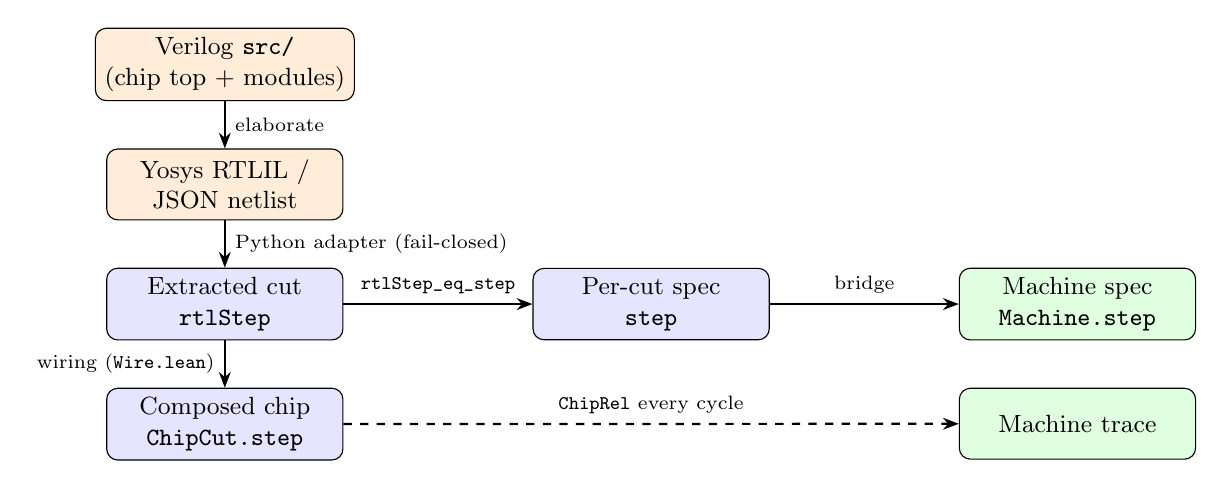
\begin{tikzpicture}[
  box/.style={draw,rounded corners,align=center,minimum width=30mm,
              minimum height=9mm,font=\small},
  arr/.style={-{Stealth[length=2mm]},thick},
  node distance=6mm and 24mm]
\node[box,fill=orange!15] (rtl) {Verilog \code{src/}\\(chip top + modules)};
\node[box,fill=orange!15,below=of rtl] (ys) {Yosys RTLIL /\\JSON netlist};
\node[box,fill=blue!10,below=of ys] (ext) {Extracted cut\\\lean{rtlStep}};
\node[box,fill=blue!10,right=of ext] (spec) {Per-cut spec\\\lean{step}};
\node[box,fill=green!12,right=of spec] (mach) {Machine spec\\\lean{Machine.step}};
\node[box,fill=blue!10,below=of ext] (chip) {Composed chip\\\lean{ChipCut.step}};
\node[box,fill=green!12,below=of mach] (mtrace) {Machine trace};
\draw[arr] (rtl) -- node[right,font=\scriptsize]{elaborate} (ys);
\draw[arr] (ys) -- node[right,font=\scriptsize]{Python adapter (fail-closed)} (ext);
\draw[arr] (ext) -- node[above,font=\scriptsize]{\lean{rtlStep_eq_step}} (spec);
\draw[arr] (spec) -- node[above,font=\scriptsize]{bridge} (mach);
\draw[arr] (ext) -- node[left,font=\scriptsize]{wiring (\code{Wire.lean})} (chip);
\draw[arr,dashed] (chip) -- node[above,font=\scriptsize]{\lean{ChipRel} every cycle} (mtrace);
\end{tikzpicture}
\caption{Proof layers. Orange: trusted inputs. Blue: RTL-derived Lean
objects. Green: specification. The dashed arrow is the headline theorem.}
\label{fig:layers}
\end{figure}

\begin{table}[!ht]
\centering\small
\begin{tabular}{@{}llrr@{}}
\toprule
Layer & Location & Files & Lines \\
\midrule
Per-cut specifications and equivalences & \code{Metronome/*.lean} & 24 & 14\,442 \\
Executable machine specification & \code{Metronome/Machine/} & 17 & 2\,486 \\
Bridges (cut $\to$ machine) & \code{Metronome/Bridge/} & 12 & 16\,388 \\
Chip composition and relation & \code{Metronome/ChipCut/} & 6 & 3\,162 \\
Premise discharge and assembly & \code{Metronome/ChipCut/Discharge/} & 20 & 22\,623 \\
\midrule
Extraction, checkers, coverage (Python) & \code{code/tests/lean/*.py} & 19 & 18\,095 \\
\bottomrule
\end{tabular}
\caption{Size of the development (Lean 4.35.0, core libraries only, no Mathlib).}
\end{table}

%======================================================================
\section{Getting the RTL into Lean: per-module cuts}
\label{sec:cuts}

\subsection{Elaboration and extraction}

The RTL is never transcribed by hand at the module level. Each checker script
runs Yosys (0.70+190) on the actual sources:
\begin{lstlisting}[language={}]
read_verilog -I src <src/*.v>
hierarchy -check -top tt_um_brentius_metronome
proc; opt_clean; write_json design.json
\end{lstlisting}
A shared Python RTLIL adapter (\code{rtlil.py}) then walks the cell graph
backwards from the chosen register inputs. It emits a Lean function
\lean{rtlStep : State -> Input -> State} built from those cells. The adapter
is \emph{fail-closed}: an unsupported cell type, a bus that cannot be resolved
to slices or bit assemblies, a missing driver or a second driver aborts the
extraction. It does not guess. The supported vocabulary is small: whole buses,
slices, bit assembly, scalar logic, equality and inequality, addition and
subtraction, unsigned comparison, indexed shifts, muxes and \code{\$pmux}, plus
the register forms used by the design.

\subsection{Cuts and free leaves}

A \emph{cut} is a set of registers together with the combinational cone that
feeds them. Nets entering the cone from outside the cut are bound as
\emph{free per-cycle inputs} (``free leaves''). Treating a driven net as
unconstrained over-approximates the circuit. This is sound for every property
the cut proves, because the proof must hold for all values of the leaf,
including the one the real driver produces. Each leaf is later
\emph{closed}: some other cut proves its driver, or the composition supplies
it (Section~\ref{sec:coverage}).

The adapter also makes structural checks where a full cone is not needed. One
example is the chip-top host filter. The checker requires
\code{cfg\_host\_now} to be exactly
\code{u\_host.wr \& in\_cfg \& live}, built from scalar \code{\$and} cells with
the leaves in that order. An OR gate or a bypass at the root therefore fails
the check.

\subsection{The equivalence theorem}

For each cut, a hand-written specification \lean{step} restates the relevant
SPEC clauses as a pure function. A template (\code{*Equivalence.lean.in}) then
receives the generated \lean{rtlStep} and proves:
\begin{lstlisting}
theorem rtlStep_eq_step (state : State) (input : Input) :
    rtlStep state input = step state input := by
  obtain (*⟨*)wr, bitc(*⟩*) := state
  obtain (*⟨*)resetN, sck, sckPrev, csN, st, isRd(*⟩*) := input
  by_cases count : bitc = 7 <;> by_cases data : st = 3 <;>
    cases resetN <;> cases sck <;> cases sckPrev <;> cases csN <;> cases isRd <;>
    simp [rtlStep, step, wrNext, bitcNext, count, data] <;> rfl
\end{lstlisting}
This is the host-write cut. Small cuts close by case analysis and reduction.
Wide datapaths (address decode, 15-bit move words, byte packing) use
\code{bv\_decide}, which bit-blasts the goal and checks an LRAT certificate.
Equality lifts to traces by induction with a generic \lean{run_congr}:
\begin{lstlisting}
theorem rtlStateAt_eq (inputs : Nat (*→*) Input) (initial : State) (n : Nat) :
    rtlStateAt inputs initial n = stateAt inputs initial n :=
  run_congr (fun state input => rtlStep_eq_step state input) inputs initial n
\end{lstlisting}
Every property proved on the specification (spacing, service, overrun,
mutual exclusion) then transfers to the RTL by rewriting with this equation.

\paragraph{Cycle convention.} The state is sampled around a rising edge.
\lean{stateAt inputs initial n} is the register state during cycle $n$. Reset
is the sampled \code{rst\_n} input of that cycle. Asynchronous clears, such as
the configuration stage's \code{we1}, are modelled as applied before the
combinational evaluation of the same cycle. The reset synchroniser is a cut of
its own (\code{rst\_m}, \code{rst\_q}).

\subsection{The cuts}

The cuts (17 checker scripts plus four cuts inside \code{verify.py}) cover
the design:
configuration arbiter and write stage; host write strobe and bit counter;
host/core configuration address decode; core pending-write queue; 480-byte
latch bank; SPI command framing; core control (\code{w\_cw} pick, freeze);
host write map; host read path and MISO; SPI pin synchronisers; data-RAM
arbiter (elaborated with \code{-D USE\_IHP\_SRAM}, so it sees the macro
boundary); threads; streams (instantiated with \code{CAP=1} and \code{CAP=0});
counters, shifters, LFSRs and accumulator; move resolution; pin lines; the two
\code{md2\_core} instances; chip-top debug, replay, program-memory and reset;
glue (sources, guards, flags, IRQ, output pins); and the op-strobe network
(\code{Strobes}).

\subsection{Mutation testing of the extraction}

A proof that the extracted function equals the specification is only as useful
as the extractor's fidelity to the RTL. To test fidelity directly, each
checker has a \code{--mutations} mode. It copies \code{src/} to a temporary
directory, plants a specific semantic fault (a swapped priority, a missing
drain clear, a wrong latch gate, early TX, a polarity flip, and so on), reruns
elaboration, extraction and proof, and requires the proof to \emph{fail} at
the intended layer. The repository is never touched. In the canonical combined
run (\code{data/raw/lean\_full\_v4\_20261121c/}) all 18 baselines were accepted
and all 129 planted faults were rejected, none accepted. Where a generated Lean
source is byte-identical to an accepted case, the proof is reused within the
run, but the source hash is regenerated for every case.

\subsection{Axiom audit}

Each emitted proof ends with
\begin{lstlisting}
/-- info: 'Metronome.Host.rtlStep_eq_step' depends on axioms: [propext, Classical.choice, Quot.sound] -/
#guard_msgs in #print axioms rtlStep_eq_step
\end{lstlisting}
so a new axiom, a \code{sorryAx} or a native certificate appearing where none
is expected fails the build. The project builds with
\code{-DwarningAsError=true}.

%======================================================================
\section{The specification side}

\subsection{An independent executable machine}

\code{Metronome/Machine/} is a cycle-level executable specification of the
whole chip, \lean{Machine.step : State -> PinIn -> State}. It was transcribed
from SPEC\_V2 and does not read the RTL. It is compiled into an executable
(\code{machine-sim}) and run in per-cycle lockstep against the Python reference
model (\code{code/tests/machine\_lockstep/}). The harness compares the pins and
a 197-key architectural state dump after every cycle, over the directed v2,
v3 and v4 scenarios plus random seeds. The final run passed all 25 lockstep tests
(\code{data/raw/lean\_machine\_lockstep\_20261122/}).

This gives the specification two independent anchors. The proof relates it to
the RTL, and lockstep relates it to the Python model, which was written
separately again. A transcription error in the machine therefore shows up
either as an unprovable step in the refinement or as a lockstep mismatch.

\subsection{Recording specification ambiguities}

Where SPEC\_V2 was silent or open to more than one reading, the machine takes
the most literal reading and marks the place with \code{-- AMBIG(n)}.
\code{Machine/AMBIGUITIES.md} lists each clause, the reading taken and the
alternatives. Several ambiguities were later \emph{closed by proof}: the
composition shows the corner is unreachable or unobservable, and a Lean
witness records why (AMBIG~1/2, 11, 14, 19).

%======================================================================
\section{Bridges: from cuts to the machine}

Each cut has its own state record. The machine has one global state. A
\emph{bridge} gives an abstraction function from the cut state to the
corresponding machine component (\lean{Bridge.Line.absSt},
\lean{Bridge.Thread.absState}, \dots), and proves a step lemma. If the cut
state abstracts to the machine component, and the cut's free leaves agree with
what the machine computes for them, then one step preserves the abstraction.

Bridges are where the cycle conventions of the two models meet. The RTL
registers a value one cycle before the machine exposes it, or keeps a copy that
the machine recomputes, or holds a value in an unread slot. The bridges absorb
these differences with explicit relations, not by weakening the claim. One
example is \lean{Bridge.StreamB.AbsRelB} for the stream capture buffer.

%======================================================================
\section{Composition: the chip model and \texorpdfstring{\code{ChipRel}}{ChipRel}}

\subsection{The product state and the wiring}

\path{ChipCut/State.lean} defines the product of all cut states plus memory
contents. \path{ChipCut/Wire.lean} builds every cut's input record from the
product state and the pins, following \code{project.v} line by line (bus
packers, byte strobes, group picks, gates). \path{ChipCut/Step.lean} then
defines \lean{ChipCut.step}. The wiring is the one hand-written view of the
chip top in the development, so every field cites the \code{project.v} line
that drives it. Section~\ref{sec:findings} lists the eight errors the proofs
found in it.

\subsection{The relation}

\lean{ChipRel s m} is a structure with 25 fields relating the product state
\lean{s} to a machine state \lean{m}:
\begin{lstlisting}
structure ChipRel (s : State) (m : Machine.State) : Prop where
  rstM : s.rst.rstM = m.r1
  lines : (*∀*) l : Fin 4, m.lines[l] = Bridge.Line.absSt (lineAt s l.val)
  threads : (*∀*) t : Fin 6, m.threads[t] = Bridge.Thread.absState (threadAt s t.val)
  streams : (*∀*) k : Fin 2, Bridge.StreamB.AbsRelB (k.val == 0) (streamAt s k.val) m.streams[k]
  p0 : P0Rel m.p0 s.p0
  cw : CwRel m.cw s.cq s.arb
  bank : BankRel s.bank m.cfg
  out : m.out = s.outPins
  oen : m.oen = s.oenPins
  -- ... 16 further fields
\end{lstlisting}
Most fields are equalities. Three are \emph{validity-guarded}, because the two
models differ only in a slot nobody reads. The P0 \code{stale} flag is compared
only while \code{land} is set. The bank-port address and data are compared only
while \code{bwp} is set. The latch bank relation says that bytes without a
latch read zero and latched bytes equal the machine's configuration byte.
\lean{pins_of_rel} projects the relation onto the driven pins:
\lean{pinsOf s = Machine.pinsOut m}.

\subsection{One step, then the trace}

The composition is a standard forward-simulation argument, in three theorems:
\begin{enumerate}
\item \lean{chip_reset_refines_rel}: on a reset cycle, \lean{ChipRel} is
  preserved with \emph{no} premises.
\item \lean{chip_step_refines'}: on an active cycle, \lean{ChipRel} and a list
  of reachable-state invariants imply \lean{ChipRel} after one step.
\item \lean{trace_refines'}: induction over $n$, with every invariant proved
  at reset and preserved by each step.
\end{enumerate}

The invariants carried along the trace are \code{Inv}, \code{AbsInv},
\code{ExecInv}, \code{HostPinInv}, \code{ldModeInv}, \code{LandingP0},
\code{LandingStream}, \code{laneInv}, \code{CapInv}, \code{streamShapeInv},
\code{StreamRelX} and \code{WindowQuiet}. Each has a \lean{_reset} lemma and
a \lean{_step} lemma, and the trace theorem threads them through together.

%======================================================================
\section{Premise discharge}
\label{sec:discharge}

\subsection{The problem}

Composing the bridges produces a large number of \emph{local premises}. Each
says that a cut's free leaf, as wired in \code{Wire.lean}, equals what the
machine computes for the corresponding signal. Early versions of
\lean{chip_step_refines} took all of these as one hypothesis structure,
\lean{Premises s m pin}. A theorem with an unproved premise structure is only
as strong as the premise, and a premise can be false (Section~\ref{sec:vacuity}).
The goal of the discharge phase was to prove every premise from the relation
and the invariants, or else move it into a short, named list.

\subsection{Named wiring hypotheses}

Discharge was organised by subsystem: line and thread, core and units, glue,
memory, host and configuration, stream and debug, move fabric, host pins,
configuration window, bank. Each subsystem got its own file in
\code{ChipCut/Discharge/}. The method was the same in each:
\begin{enumerate}
\item State each missing fact as a \emph{named} wiring hypothesis over the
  current related states, for example ``the stream's effective mode on this
  cycle equals the machine's mode''. A temporary structure
  (\code{OpenWiring}) collected the hypotheses still open.
\item Prove each hypothesis in a separate wiring file (\code{LineMoveWire},
  \code{StreamMoveWire}, \code{CoreCombWire}, \code{MovePayloadWire},
  \code{DbgMapWire}, \code{BankWire}, \code{WindowWire}, \code{PremiseWire},
  \dots) from \code{Wire.lean}, the cut equations and the invariants.
\item Delete the field from \code{OpenWiring} once proved. The phase is
  finished when the structure is gone. \code{\#print OpenWiring} was used as the
  check for what remained.
\end{enumerate}

\subsection{Projected forms, kept honest by counter-witnesses}

Some relations hold only on the bits the machine actually reads, not on whole
registers. Where a field was restated in projected (low-bit) form, the
development also proves that the \emph{exact} form is false on a reachable
state. A weakening is therefore always justified by a concrete counterexample,
and never made just because the stronger form was hard to prove. Examples:
\lean{capWb_reachable_witness}, \lean{streamWire_landing_false},
\lean{frozen_landing_invalid_nv_disagrees} and
\lean{contents_open_cbs_counterexample}.

\subsection{Constant tables}

Eight decode tables map instruction fields to names: sources, guards, jump
guards, destination kind, destination payload, FLAGS/P0/CW codes, ports, and
stream and line codes. They are closed propositions over string-named
entries. Lean's kernel cannot reduce the parsed string names efficiently, so
each table proposition is checked by \emph{compiled} evaluation
(\code{decode\_check\_*.lean}, 0 failures for all eight) and enters the
theorem as the hypothesis \lean{Tables}. This is a deliberate trust decision:
it is recorded in the statement instead of hidden behind \code{native\_decide},
which would add the \code{Lean.trustCompiler} axiom to every downstream
theorem.

\subsection{The latch bank}

The configuration bank has 480 byte slots. 284 of them are live, with 2,112
latch bits in total, and 56 bytes are only partly latched. An earlier version
assumed the bank contract. The final version generates the real
\code{CFG\_MASK} byte table from \code{src/md2\_map.vh}, with a generator that
asserts the bit count against \code{CFG\_LATCH\_BITS}. It proves that the RTL
and the machine read the same configuration byte at every offset under that
mask (\code{BankWire.lean}). The power-on condition \lean{MaskedZero} (every
implemented latch bit clear, as reset leaves them) became an initial condition.

%======================================================================
\section{Keeping the theorem non-vacuous}
\label{sec:vacuity}

A refinement theorem with hypotheses holds trivially if the hypotheses can
never be met. The development guards against this in three ways.

\paragraph{Satisfiability witnesses.} Two theorems construct concrete inputs:
\begin{lstlisting}
theorem trace_premises_satisfiable (_tables : Tables) :
    (*∃*) (pins : Nat (*→*) Machine.PinIn) (cont : Contents),
      InitialConditions cont (*∧*)
        (*∀*) n, PinPremises (cutStateAt pins (resetState cont) n) (pins n)
\end{lstlisting}
The first uses idle pins and zeroed contents. The second,
\lean{trace_premises_satisfiable_active}, releases reset, runs an active cycle
in which stream~0 raises a fetch request, then resets again. Both depend only
on the three standard axioms.

\paragraph{Witnesses for rejected premise forms.} When a premise was found to
be false at a reachable state, the falsity was proved and kept, for example
\lean{old_premise_false_at_zero}.

\paragraph{Independent review.} The capstone was reviewed twice, read-only, by
a reviewer model with no write access. The first review found the statement
\emph{vacuous}: the configuration-write release-window premise was false at
reset, so no trace satisfied the hypotheses. It also found that the latch bank
was not really modelled. The fix replaced the window premise with a proof
(\code{WindowWire.lean}: no configuration write can occur while the window is
open), modelled the bank with the real mask, relaxed a stream premise that
blocked normal start-up, and proved two premises that had been assumed. The
second review found no remaining blocker.

The lesson is general. Checking the hypotheses of a capstone theorem for
satisfiability is as important as checking the proof, and the check belongs in
Lean as a theorem, not in a reviewer's head.

%======================================================================
\section{The final statement}

\begin{lstlisting}
theorem trace_refines' (pins : Nat (*→*) Machine.PinIn) (cont : Contents)
    (tables : Tables) (initial : InitialConditions cont)
    (env : (*∀*) n, PinPremises (cutStateAt pins (resetState cont) n) (pins n)) (n : Nat) :
    ChipRel (cutStateAt pins (resetState cont) n)
            (machineStateAt pins (absChip (resetState cont)) n)
\end{lstlisting}

\begin{table}[!ht]
\centering\small
\begin{tabularx}{\linewidth}{@{}l>{\raggedright\arraybackslash}X@{}}
\toprule
Hypothesis & Content \\
\midrule
\lean{Tables} & The eight constant decode tables (compiled evaluation). \\
\lean{InitialConditions} & \code{ramOwner = 0}; \lean{MaskedZero cont.cfg};
  configuration image has the right size. \\
\lean{PinPremises}, per cycle & \lean{host_sck_spacing}: a byte-completing SCK
  edge coincides with neither a register-read acknowledgement nor a host
  data-RAM landing.\newline
  \lean{stream_mode_quiet}: a stream's effective mode changes only when it
  has no read in flight, no second replay slot and no pending byte. \\
\bottomrule
\end{tabularx}
\caption{All hypotheses of the headline theorem.}
\end{table}

\code{\#print axioms trace\_refines'} gives \code{propext},
\code{Classical.choice}, \code{Quot.sound} and 96 \code{bv\_decide} certificate
axioms. It shows no \code{sorryAx} and no \code{Lean.trustCompiler}. An
incremental build of the capstone over the already-built per-cut objects
takes about 18\,s, and the capstone is part of the default \code{lake build}
target.

%======================================================================
\section{Checks outside the proof}
\label{sec:coverage}

The proof says nothing about RTL that no cut reads. A separate inventory,
\code{coverage\_check.py}, therefore answers two questions about the real
elaboration.
\begin{description}
\item[Coverage.] Which elaborated cells does each cut's extracted cone read,
  and which cells does no cut read? It imports the 16 checker modules and
  calls their own extraction entry points, wrapping the binding methods of the
  shared adapter. It reimplements nothing.
\item[Closure.] For every net a cut leaves free, where does the net come from,
  and is its source itself proved?
\end{description}
In strict mode the inventory is a gate: any uncovered non-black-box cell or any
unclosed leaf makes it exit 1. The first inventory showed 90.74\,\% coverage,
with 830 uncovered chip-top cells in the op-strobe network and 35 unclosed
leaves. That result directly led to the \code{Strobes} cut. The final strict
run (\code{data/raw/lean\_coverage\_v4\_20261122b/}) shows 100\,\% of 8,962
cell occurrences read by a cut or a named structural check (8,959, plus 3 SRAM
macro black boxes), 633 free leaves, 0 unclosed, and all 24 output bits driven
by covered logic.

Coverage records \emph{where} each free leaf comes from. It does not compare
the \code{Wire.lean} expression for that leaf with the RTL net. That comparison
was done by hand, line by line against \code{project.v}, and it is part of the
trusted base below.

%======================================================================
\section{What the proofs found}
\label{sec:findings}

The RTL needed no change. The proofs found errors in the two hand-written
models.
\begin{itemize}
\item \textbf{Eight wiring errors in \code{Wire.lean}}, each confirmed against
  \code{project.v}:
  \begin{itemize}
  \item bus packers put item~0 in the high position;
  \item the bank was fed from the arbiter rather than the registered stage;
  \item the core thread-select polarity was wrong;
  \item the stream \code{CAP} parameter was set on both streams;
  \item the PHASE byte strobes were in the wrong order;
  \item a configuration write wrongly gated the shifter data write;
  \item the replay-valid bit order was wrong;
  \item the EMASK/RLV byte-0 strobes fired for any byte.
  \end{itemize}
  An earlier audit of the same file found ten further mismatches (for example
  the RX bit source, the data-RAM host gate and the \code{CWOVR} clear bit).
\item \textbf{One machine-spec transcription error.} \code{RLVP} must hold its
  value while frozen. The fix is one line:
  \lean{rlvp := if frozen then d.rlvp else d.rlv}.
  The proof attempt failed only on the frozen branch, and the machine lockstep
  passed 25 of 25 again after the fix.
\item \textbf{Specification corners}, each settled by a witness: AMBIG~1/2, 11,
  14 and 19.
\end{itemize}
Every wiring error made the model wrong in a way a proof would otherwise have
carried into the theorem. None of them was a simulation-visible bug in the
silicon design. That is the expected outcome: the RTL had already been through
lockstep simulation, and the formal work mainly checks the models that
describe it.

%======================================================================
\section{Trusted base and limitations}

\subsection{Trusted base}
\begin{itemize}
\item Yosys elaboration of \code{src/} (\code{proc}, \code{opt\_clean}).
\item The Python RTLIL adapter, the per-cut adapters and their structural
  checks. These are exercised, but not proved, by the 129 planted faults.
\item The hand-written chip-top wiring in \path{ChipCut/Wire.lean} and
  \code{Step.lean}.
\item The behavioural latch, clock-gate and SRAM models standing in for the
  IHP cells (\code{sg13cmos5l\_lgcp\_1}, \code{sg13cmos5l\_dlhrq\_1}, SRAM
  macros).
\item Native evaluation behind the \code{bv\_decide} LRAT certificates, and
  compiled evaluation of the eight tables.
\item The Lean~4.35.0 kernel and its three standard axioms.
\end{itemize}

\subsection{Limitations}
\begin{itemize}
\item \textbf{Sampled digital behaviour only.} There is no statement about
  timing closure at 60\,MHz, metastability of the input synchronisers, or the
  gate-level netlist. Equivalence between the netlist and the RTL needs
  separate evidence.
\item \textbf{\lean{host_sck_spacing} is stronger than the documented host
  rate.} Besides SCK $\le$ clk/16, it requires that a host RAM read does not
  land on the edge that completes a byte. Whether that holds depends on RAM
  arbitration, because S0, S1 and P0 can delay host service. SPEC~\S9's
  12-cycle service budget implies the rule, but the RTL has no unconditional
  bound.
\item \textbf{\lean{stream_mode_quiet} is stricter than SPEC~\S9a.13}, which
  only makes a mode change mid-transfer unspecified until the next rewind.
\item \textbf{The witnesses are short.} They show the hypotheses can be met for
  idle operation and a brief active start-up. They do not show sustained
  operation with SPI configuration writes and stream transfers.
\end{itemize}

%======================================================================
\section{Process notes}

The work was split into bounded tasks with owned files. Each per-module cut,
bridge and discharge file was a separate delegated task with an acceptance
check: \code{lake build} with warnings as errors, the axiom guard, a baseline
plus mutation run, and \code{src/} unchanged. An orchestrator integrated the
results, re-ran the combined checks and kept a single status record. Most of
the implementation was done by LLM coding agents. The independent reviews
were done by a different model, read-only. Two practices mattered most:
\begin{enumerate}
\item \textbf{Every weakening needs a witness.} A premise could be relaxed or a
  field projected only when the stronger form was proved false at a reachable
  state. This stopped the agents from trading correctness for progress.
\item \textbf{Evidence before claims.} Every number in this document comes from
  a retained raw log under \code{data/raw/lean\_*}: build logs, axiom dumps,
  coverage JSON and mutation status files. Each was produced by a command
  recorded beside it.
\end{enumerate}

\section{Reproducing}
From the repository root, with Elan and the OSS CAD Suite on \code{PATH}:
\begin{lstlisting}[language={}]
(cd code/tests/lean && lake build)            # cuts, bridges, capstone
python code/tests/lean/verify.py --mutations --artifacts-dir <fresh dir>
python code/tests/lean/coverage_check.py --strict --artifacts-dir <fresh dir>
(cd code/tests/lean && lake build machine-sim)
python -m pytest code/tests/machine_lockstep -q   # machine vs Python model
\end{lstlisting}
Evidence for this write-up:
\begin{itemize}
\item \code{data/raw/lean\_chipcut\_final\_v4\_20261122/}
\item \code{data/raw/lean\_coverage\_v4\_20261122b/}
\item \code{data/raw/lean\_full\_v4\_20261121c/}
\item \code{data/raw/lean\_machine\_lockstep\_20261122/}
\end{itemize}
The per-cut details are in \code{code/tests/lean/README.md}.

\end{document}
